\section{Método das Substituições Sucessivas (Iteração de Ponto Fixo)}
%\index{Método das Substituições Sucessivas (Iteração de Ponto Fixo)}

\subsection{Descrição}

Dado $f(x) \Rightarrow f(x) = 0$ rearranja-se $f(x) = 0$ na forma:

\[
 x = \overline{f}(x)
\]

Assim, pode-se escrever um método iterativo como:

\[
 x_{i} = \overline{f}(x_{i-1})
\]

\subsection{Características}

\begin{itemize}
 \item Necessita de uma estimativa incial.
 \item Tem a vantagem de ser simples.
 \item Flexibilidade na escolha de $\overline{f}$.
 \item Para garantir convergência $\overline{f'}(x) < 1$ deve ser satisfeita na vizinhança da raiz.

\begin{itemize}
 \item $0 < \overline{f'} < 1 \Rightarrow$ convergência assintótica.
 \item $-1 < \overline{f'} < 0 \Rightarrow$ convergência oscilatória.
\end{itemize}

\end{itemize}

\begin{figure}[htb]
  %\index{figura da posição falsa modificado}%
  \setlength{\abovecaptionskip}{20pt}
  %%% o valor default de \abovecaptionskip definido para a classe
  %%% article e de 10pt.
  \centering
  %%% VIDE ABAIXO COMENTARIO SOBRE USO DE DIRETORIOS NO PATHNAME
  %%% DOS ARQUIVOS INCLUIDOS.
  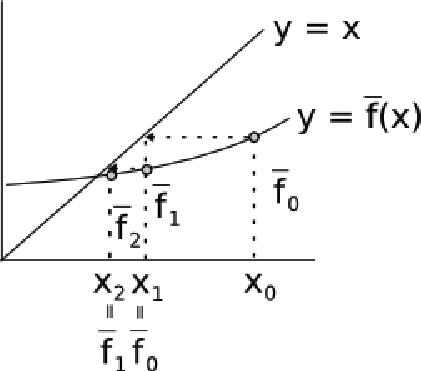
\includegraphics[scale=0.9]{capitulos/capitulo1/figuras/substituicoes1-eps-converted-to.pdf}
  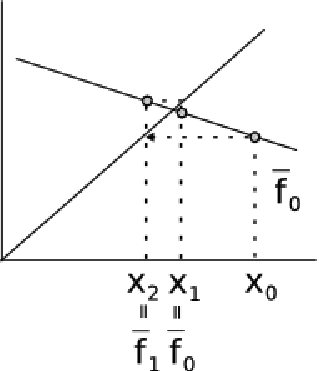
\includegraphics[scale=0.9]{capitulos/capitulo1/figuras/substituicoes2-eps-converted-to.pdf}
  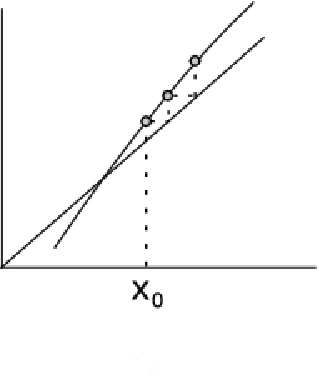
\includegraphics[scale=0.9]{capitulos/capitulo1/figuras/substituicoes3-eps-converted-to.pdf}
  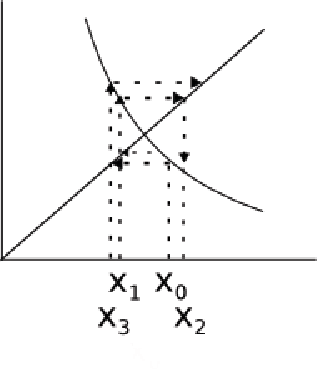
\includegraphics[scale=0.9]{capitulos/capitulo1/figuras/substituicoes4-eps-converted-to.pdf}

  \caption{Descrição do método das substituições sucessivas.}
  \label{fig:substituicoes1}  
\end{figure}

\subsection{Notas}

\begin{enumerar}
 \item Se $x_{n-2}$ e $x_{n-1}$ se tornarem muito próximos, $y_{n-2}$ e $y_{n-1}$ também se tornam próximos e erro de arredondamento significativo ocorre na divisão $ \displaystyle \frac{x_{n-1} - x_{n-2}}{f_{n-1} - f_{n-2}} $. Para evitar isso:

\begin{itemize}
 \item Quando $ |f_{n}| < \Delta$:

 \begin{enumerar}
 \item congela-se $x_{n-2}$ e $y_{n-2}$

 \item ou $x_{n-2}$ e $f_{n-2}$ são trocados por $x_{n-2} + \xi$ é $f(x_{n-2} + \xi)$ onde $\xi$ é pequeno mas suficientemente grande para evitar erro de arredondamento.
 \end{enumerar}

\end{itemize}

 \item O método pode divergir ou convergir para uma solução irrelevante se as aproximações iniciais não forem boas.

 \item O método é uma variação, computacionalmente mais eficiente, do método de Newton.

 \end{enumerar}

\begin{example}
\label{ex:substituicoes1}

 $f(x) = x^{2} - 3 \ast x + e^{x} - 2$ tem duas raízes, uma negativa e outra positiva. Encontre a menor raiz pelo método das substituições sucessivas.

\textbf{Solução:}

\begin{enumerate}

\item Tente determinar um intervalo que contém a raiz:

\begin{itemize}
 \item Para $x = 0 \Rightarrow f(0) = -1$.
 \item Para $x = -1 \Rightarrow f(-1) = 2.367$.
 \item Se $f(x)$ for contínua nesse intervalo a curva cortará o eixo dos $x$.
\end{itemize}

\item Reescreva $f(x) = 0$ na forma $x = \overline{f}(x)$:
\[
 x^{2} - 3 \ast x + e^{x} - 2 = 0 \Rightarrow x = \frac{x^{2} + e^{x} -2}{3}
\]

\item Método iterativo:

\[
 x_{i} = \frac{x_{i-1}^{2} + e^{x_{i-1}} -2}{3}
\]

onde $ \displaystyle \overline{f}(x) = \frac{x^{2} + e^{x} -2}{3}$

\item Verifique condição de convergência $|\overline{f'}(x) | < 1$

\[
 \overline{f'}(x) = \frac{1}{3} \ast (2 \ast x + e^{x})
\]
\[
 -1 < \frac{1}{3} \ast (2 \ast x + e^{x}) < 1
\]
\[
 \Rightarrow -3 < \frac{1}{3} \ast (2 \ast x + e^{x}) < 3
\]
\[
 \forall x \in [-1,0] \Rightarrow -1.63 \leq 2 \ast x + e^{x} \leq 1
\]

\underline{Conclusão:} O critério é convergente no intervalo.

\item Aplique o método iterativo com $x_{0} = 0$.

\begin{table}[htp]
\footnotesize
	\centering
		
		\begin{tabular}{|c|c|}
		\hline		
		\textbf{$n$} & \textbf{$x_{n}$}\\
		\hline \hline 
		0 & 0\\
		\hline 
		1 & -0.333333\\
		\hline 
		2 & -0.390786\\
		\hline 
		3 & -0.390254\\
		\hline
		4 & -0.390272\\
		\hline
		5 & -0.390272\\
		\hline
		\end{tabular}
	%\caption{Iterações do método da bisseção}
	\caption{Exemplo de iterações do Método das Substituições Sucessivas.}
	\label{tab:sucessivo1}
\end{table}

\underline{Resposta:} Solução de $f(x) = 0$

$x = -0390272$ (ver tabela \ref{tab:sucessivo1})

Outras opções para $\overline{f'}(x):$

\[
 x = - \sqrt{3 \ast x - e^{x} + 2}
\]

e

\[
 x = \sqrt{3 \ast x - e^{x} + 2}
\]

\[
 \overline{f'}(x) = \pm \frac{1}{2} \ast \frac{3 - e^{x}}{\sqrt{3 \ast x - e^{x} + 2}}
\]

Para $x = 0 \Rightarrow \overline{f'}(0) = \pm \frac{1}{2} \ast \frac{3 - 1}{\sqrt{1}} = \pm 1$
\[
 x= -1 \Rightarrow \overline{f'}(-1) = \pm \frac{1}{2} \ast \frac{1}{2} \ast \frac{3 - e^{-1}}{\sqrt{-3 - e^{-1} + 2}} = \pm \frac{1.32}{\sqrt{-1.37}}
\]

Critério de convergência não é satisfeito.

$\overline{f'}(x)$ é singular na vizinhança da raiz.

\end{enumerate}

\end{example}

\subsection{Forma sistemática de encontrar $\overline{f'}(x)$}

\[
 \bar{f}\,(x) = x - \alpha \, f \, (x) \Rightarrow \bar{f}\,(x) = 1 - \alpha \, f'\,(x)
\]

Assim, o esquema iterativo pode ser escrito como

\[
 \mbox{ \framebox{ $ x_n = x_{n-1} - \alpha \, f\,(x_{n-1}) $ } } \qquad (*)
\]

onde \esp{\alpha = constante}.

OBS: Se o esquema converge, \esp{x} satisfaz \esp{f(0) = 0}.

Critério de convergência:

\[
-1 < 1 - \alpha \, f'(x) < 1
\]

ou

\[
 \mbox{ \framebox{ $ 0 < \alpha \, f'(x) < 2 $ } } \qquad (**)
\]

\begin{itemize}
 \item \esp{\alpha} deve ter o mesmo sinal de \esp{f'(x)}
 \item para \esp{\alpha \approx 0 \Rightarrow} (*) sempre converge
 \item se \esp{\alpha \approx \displaystyle \frac{1}{f'(x)} \, \, * \underbrace{h}_{\mbox{\textit{\scriptsize{para cada iteração}}}}} , a convergência é ótima e o método se reduz ao método de Newton.
\end{itemize}

\begin{example}
Seja 

\[
 f\,(x) = \tan\,(0.1\,x) - 9.2 \, e^{-x}
\]


Determine a menor raiz positiva sabendo-se que ela se encontra em \esp{[3,\,4]}

\textbf{Solução:}

\begin{itemize}
 \item Aproximação de $f'$ no intervalo \esp{[3,\,4]}:
 \esp{
  \begin{array}{ll}
   f' & = \displaystyle \frac{f\,(4) - f\,(3)}{4-3} = 0.40 \\
   \\
      & = 0.40299
  \end{array}
 }

 \item \esp{\alpha \approx \displaystyle \frac{1}{f'} = \frac{1}{0.40299} = 2.4814}

 \item \esp{x_n = x_{n-1} - 2.4814 \, [\tan\,(0.1\,x) - 9.2\,e^{-x}]}

\end{itemize}

\begin{table}[htp]
\footnotesize
	\centering
		
		\begin{tabular}{|c|c|}
		\hline		
		\textbf{$n$} & \textbf{$x_{n}$}\\
		\hline \hline 
		0 & 4\\
		\hline 
		1 & 3.36899\\
		\hline 
		2 & 3.28574\\
		\hline 
		3 & 3.29384\\
		\hline
		4 & 3.28280\\
		\hline
		5 & 3.29293\\
		\hline
		6 & 3.29292\\
		\hline
		7 & 3.29292\\
		\hline
		\end{tabular}
	%\caption{Iterações do método da bisseção}
	\caption{Exemplo de Forma sistemática de encontrar $\overline{f'}(x)$.}
	\label{tab:sucessivo2}
\end{table}

\[
 x = 3.29292
\]

\end{example}

\textbf{Nota:} O método de Newton e o método da Secante são casos particulares do método das substituições sucessivas.